\documentclass{article}

\usepackage[T1]{fontenc}
\usepackage{svninfo}
\usepackage{graphicx}
\usepackage[round]{natbib}
\usepackage{verbatim}
\usepackage{caption}
\usepackage{subcaption}
\usepackage{times}
\usepackage{authblk}

\begin{document}

\bibliographystyle{abbrvnat}

\svnInfo $Id$

\newcommand{\dbatversion}{0.2}

\title{The Damped Bundle Adjustment Toolbox\\v\dbatversion{} for Matlab}

\author[1]{Niclas B{\"o}rlin}
\author[2]{Pierre Grussenmeyer}
\affil[1]{Department of Computing Science, Ume{\aa} University,
  Sweden, \texttt{niclas.borlin@cs.umu.se}}
\affil[2]{ICube Laboratory UMR 7357, Photogrammetry and Geomatics Group, INSA Strasbourg, France}
\date{\today}

\maketitle

\newpage

\tableofcontents

\newpage

\section{Introduction}

\subsection{Purpose}

This purpose of the Damped Bundle Adjustment toolbox is to be a
high-level toolbox for photogrammetry in general and bundle adjustment
in particular. It is the hope of the authors that the high-level
nature of the code will inspire algorithm development. The code is
written in Matlab and is verified to work with Matlab version 8
(release R2012B). The intention is that at least the computation
routines will be Octave-compatible. This has however not been tested
yet.

\subsection{Capabilities}

The toolbox currently includes routines for (function names in parentheses):
\begin{itemize}
\item File handling:
  \begin{itemize}
  \item Reading Photomodeler-style text export files (\texttt{loadpm}).
  \item Writing Photomodeler-style text result files
    (\texttt{bundle\_result\_file}).
  \end{itemize}
\item Photogrammetric calculations, including:
  \begin{itemize}
  \item Spatial resection (\texttt{resect}).
  \item Forward intersection (\texttt{forwintersect}).
  \item Relative orientation based on the Nist{\'e}r 5-point algorithm
    \citep{Stewenius2006:Recent} will be added in the future.
  \end{itemize}
\item Bundle adjustment
  \begin{itemize}
  \item Bundle adjustment proper (\texttt{bundle}) using either
    Classical, Gauss-Newton-Armijo, Levenberg-Marquardt, or
    Levenberg-Marquardt-Powell damping schemes
    \citep{Borlin2013:Bundle}. The latter two damping schemes are so
    far not included. They will be added in the near future, as will
    chirality damping.
  \item Covariance calculations (\texttt{bundle\_cov}) from the bundle
    result.
  \end{itemize}
\item Various plotting functions, including:
  \begin{itemize}
  \item Plot image area covered by measurements
    (\texttt{plotcoverage}).
  \item Plot camera network (\texttt{plotnetwork}), either static
    (as-loaded) or as an illustration of the bundle iterations.
  \item Plot of the iteration trace of parameters estimated by bundle
    (\texttt{plotparams}).
  \item Plots of quality statistics from the bundle result
    (\texttt{plotimagestats, plotopstats}).
  \end{itemize}
\item Demo functions using the above functions. The demo functions are
  detailed in Section~\ref{sec:demos}.
\end{itemize}

This manual does not contain detailed information about how to use
each function. More information may be found by typing \texttt{help
  <function name>} at the Matlab prompt, studying the source code of
the demo functions, and reading the source code of each file directly.

Things to be added in the near future:
\begin{itemize}
\item Weights on the observations.
\item Chirality damping.
\item Levenberg-Marquardt and Levenberg-Marquardt-Powell damping.
\item Test octave compatibility.
\item Azimuth-tilt-swing camera model.
\end{itemize}

\subsection{Legal}

The licence detail are described in the \texttt{README.txt} file
included in the distribution. In summary:
\begin{itemize}
\item You use the code at your own risk.
\item You may use the code for any purpose, including commercial, as
  long as you give due credit. Specifically, if you use the code, or
  derivatives thereof, for scientific publications, you should refer
  to on or more of the papers
  \citet{Borlin2013:Bundle,Borlin2013:Experiments} that the code is
  based on.
\item You may modify and redistribute the code as long as the
  licensing details are also redistributed.
\end{itemize}

\section{Installation}
\label{sec:install}

\begin{enumerate}
\item Download the package file {\tt
  \verb+dbat_+\dbatversion\verb+.zip+}.
\item Unpack the package into a directory \emph{dbat}.
\item \label{step:dbatInit}
Inside Matlab, do the following initialization:\\
\verb+cd dbat % the directory where you installed the files.+\\
\verb+dbatSetup % set paths, etc.+
\item Test the installation by executing the supplied demos described
  in Section~\ref{sec:demos}.
\end{enumerate}

\section{Usage}

\subsection{Demos}
\label{sec:demos}

\subsubsection{loadplotdemo}
\label{sec:loadplotdemo}
\label{sec:loadroma}

The \verb+loadplotdemo+ demo loads a modified Photomodeler text export
file of the 60-camera, 26000-point project used
in~\citet{Borlin2013:Bundle}. The camera network, as computed by
Photomodeler, is plotted with camera 1 aligned to the cardinal axes.
The result should look like Figure~\ref{fig:roma}. The figure is a
standard Matlab 3D figure and may e.g.\ be rotated or zoomed using the
camera toolbar.

\begin{figure*}
  \centering
  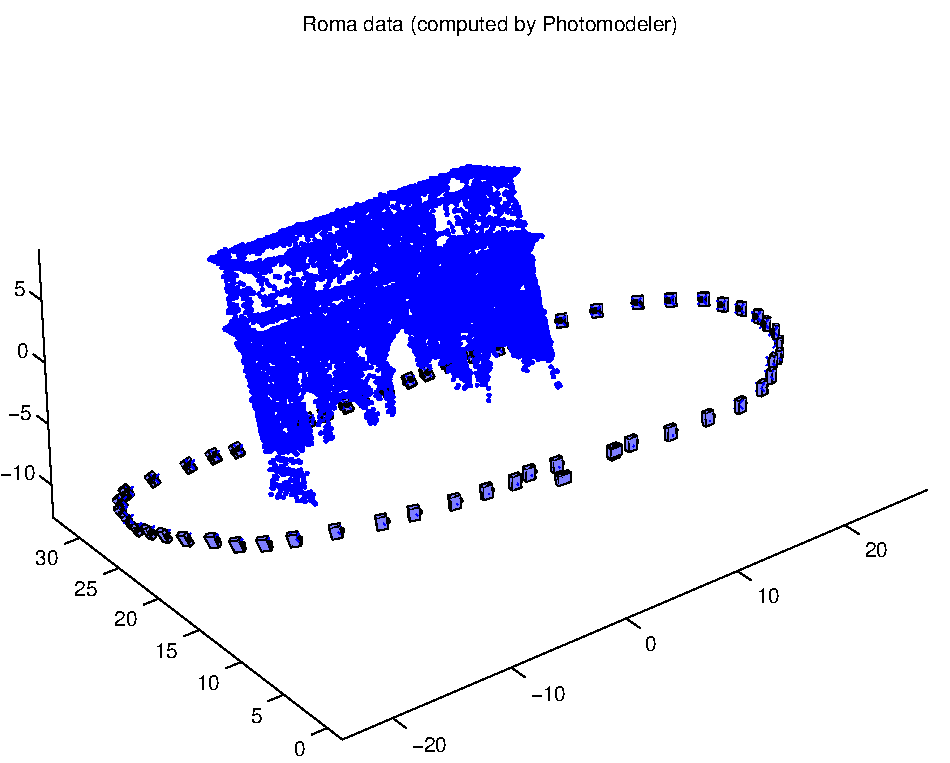
\includegraphics[width=0.5\hsize]{ill/roma}
  \caption{The figure generated by the \texttt{loadplotdemo} demo.}
  \label{fig:roma}
\end{figure*}

\subsubsection{loadplotdemo2}
\label{sec:camcaldata}

The \verb+loadplotdemo2+ demo loads a modified Photomodeler text
export file of a 21-camera, 100-point camera calibration project. The
camera network, as computed by Photomodeler, is plotted and should
look like Figure~\ref{fig:camcalib}. The figure is a standard Matlab
3D figure and may e.g.\ be rotated or zoomed using the camera toolbar.

\begin{figure*}
  \centering
  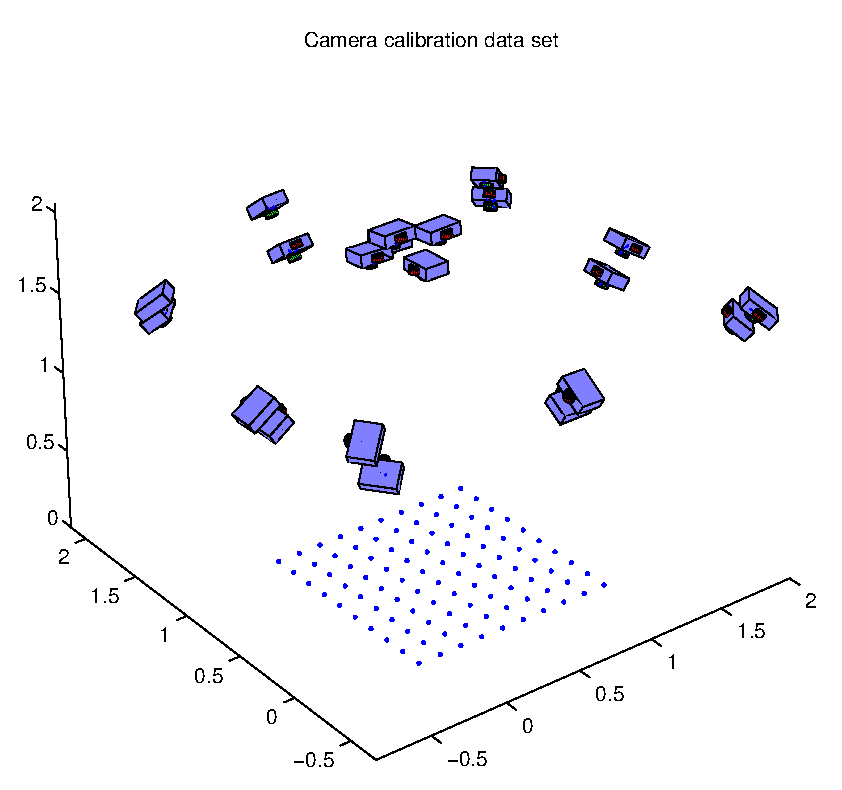
\includegraphics[width=0.5\hsize]{ill/ccam}
  \caption{The figure generated by the \texttt{loadplotdemo2} demo.}
  \label{fig:camcalib}
\end{figure*}

\subsubsection{camcaldemo}

The \verb+camcaldemo+ demo loads the camera calibration export file
from Section~\ref{sec:camcaldata} and runs a camera calibration. The
EXIF focal length is used as the initial value. The other values are
set to ``default'' values, e.g.\ the principal point at the center of
the sensor and all lens distortion parameters equal to zero. The
initial value for the EO parameters are computed by spatial
resection~\citep[Chap.~11.1.3.4]{Haralick1994:Review,McGlone2004:Manual} using
the control points defined for the Photomodeler calibration sheet. The
initial OP coordinates are subsequently computed by forward
intersection.

The bundle adjustment is run with Gauss-Newton-Armijo damping. The
result is given in a number of plot windows and a Photomodeler-style
result text file. The result plots are of two kinds: Plots that show
the evolution of the iterations and plots that show the quality of the
input or output data. The former plots may be useful to understand how
the bundle adjustment works but also to ``debug'' a difficult network
that has convergence difficulties. The latter plots give information
about the quality of the result and may also provide clues on how to
improve a network when the bundle did converge.

\paragraph{Evolution plots}

\begin{figure*}
  \centering
  \begin{subfigure}[b]{0.49\textwidth}
    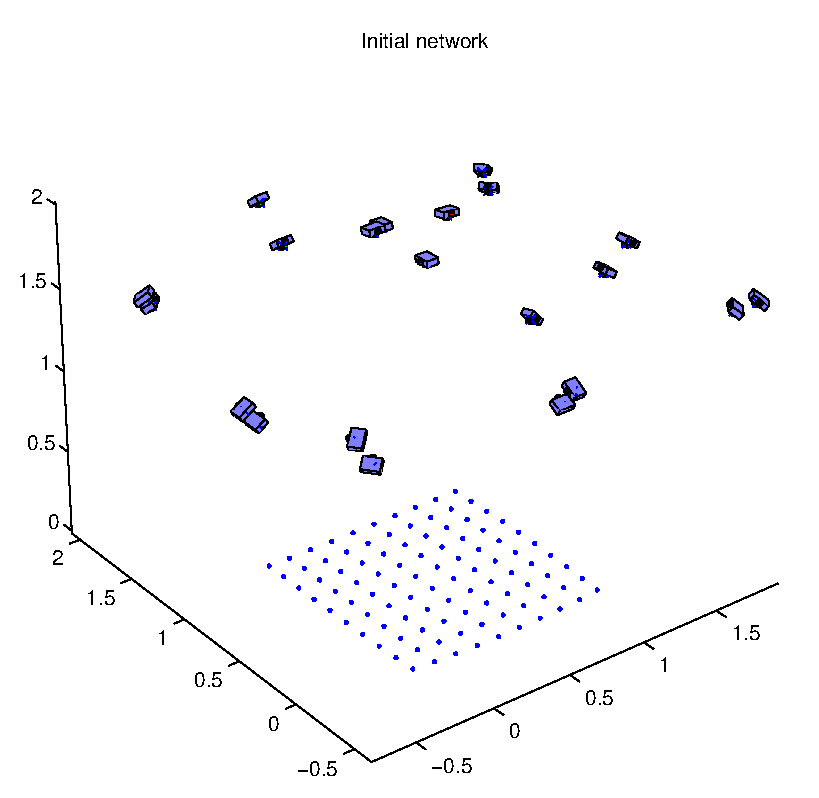
\includegraphics[width=\textwidth]{ill/ccamx0}
    \caption{Initial network configuration.\\~}
    \label{fig:camx0}
  \end{subfigure}%
  \begin{subfigure}[b]{0.49\textwidth}
    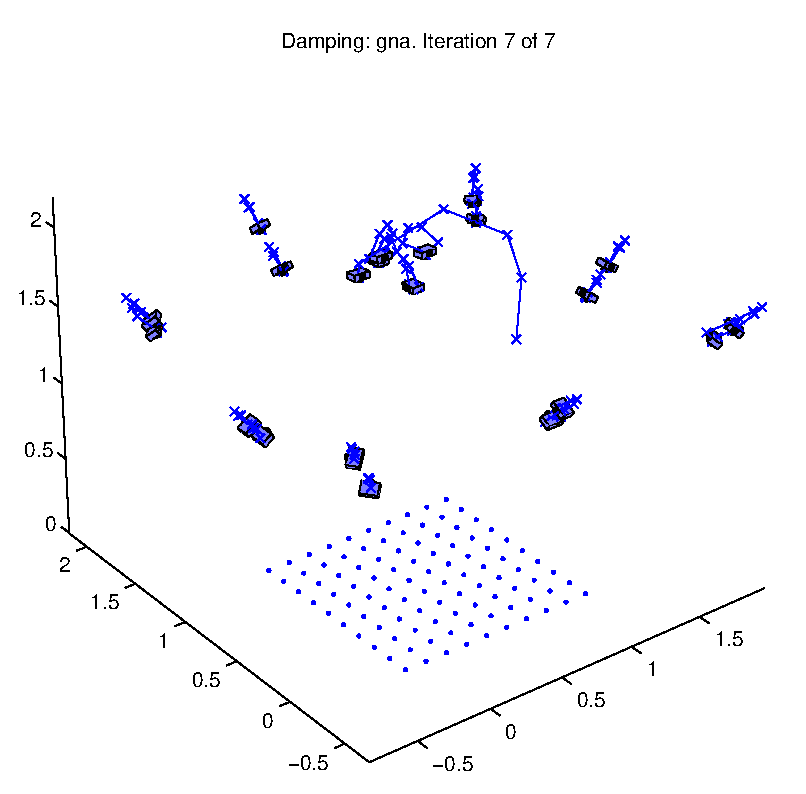
\includegraphics[width=\textwidth]{ill/ccamxfinal}
    \caption{Network configuration after convergence, with camera
      center trace lines.}
    \label{fig:camxfinal}
  \end{subfigure}
  \caption{3D network evolution during the iterations. Only the EO and
    OP parameters are illustrated. In this example, the variation of
    the OP coordinates is barely visible. }\label{fig:net3DTrace}
\end{figure*}

The evolution plots are collected in
figures~\ref{fig:net3DTrace}--\ref{fig:gnatrace}.
Figure~\ref{fig:net3DTrace} shows a snapshot of the 3D trace figure at
the beginning and end of the iterations. As default, the evolution is
presented iteration by iteration with intervening presses of the
return key. The figure window is interactive and may be rotated,
zoomed, etc. In this example, it is clear in
Figure~\ref{fig:camxfinal} that one camera station had poorer initial
values than the rest.

\begin{figure*}
  \centering
  \begin{subfigure}[b]{0.3\textwidth}
    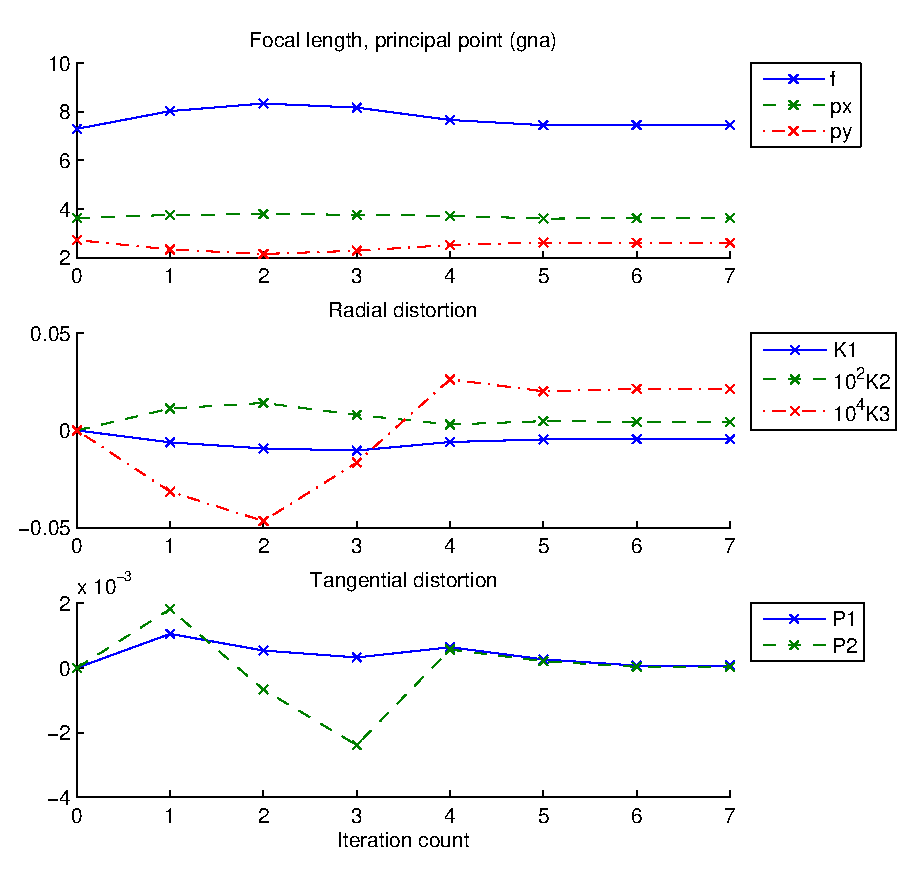
\includegraphics[width=\textwidth]{ill/ccamiotrace}
    \caption{IO parameters}
    \label{fig:IOtrace}
  \end{subfigure}%
  \begin{subfigure}[b]{0.3\textwidth}
    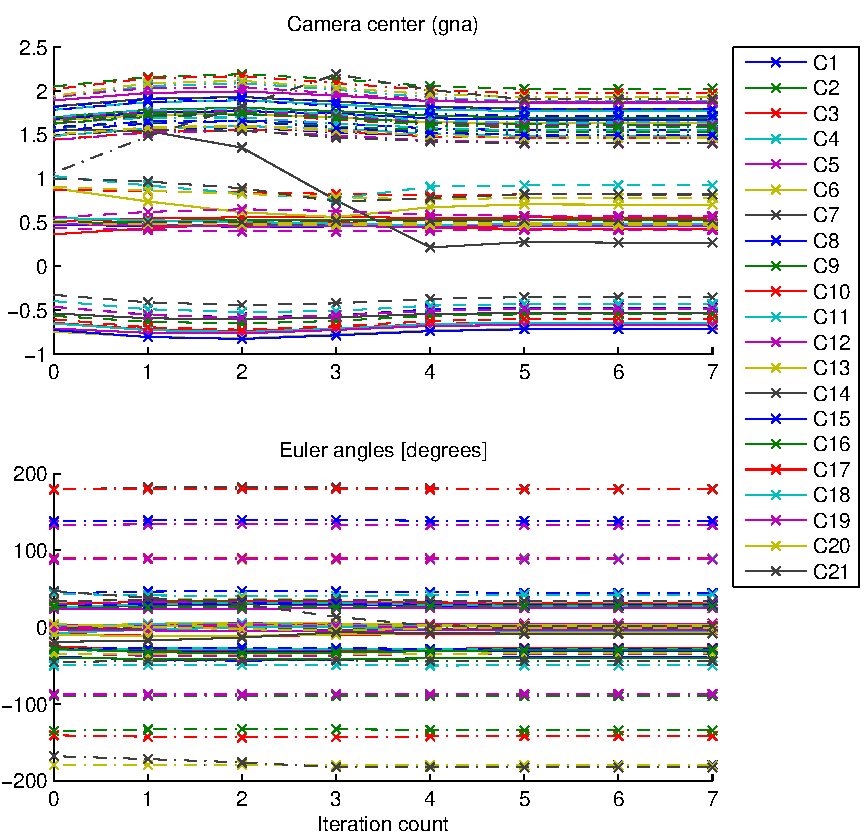
\includegraphics[width=\textwidth]{ill/ccameotrace}
    \caption{EO parameters}
    \label{fig:EOtrace}
  \end{subfigure}
  \begin{subfigure}[b]{0.3\textwidth}
    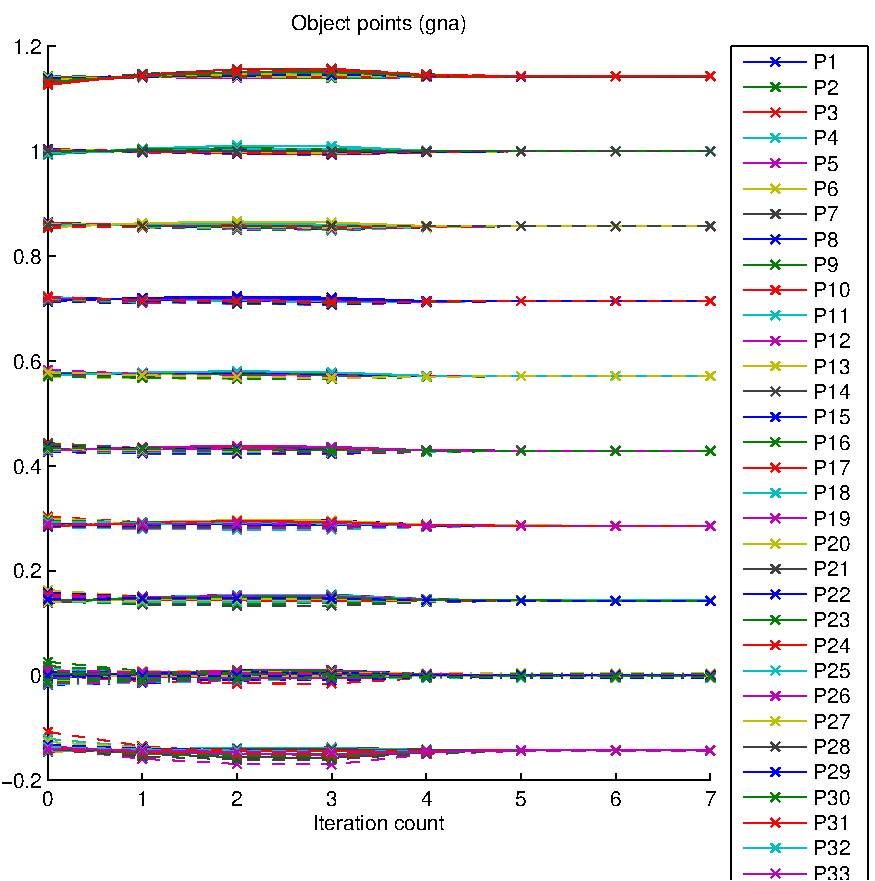
\includegraphics[width=\textwidth]{ill/ccamoptrace}
    \caption{OP parameters}
    \label{fig:OPtrace}
  \end{subfigure}
  \caption{Evolution of network parameters during the iteration
    sequence.}\label{fig:netTrace}
\end{figure*}

Figure~\ref{fig:netTrace} contains three plots showing the evolution
of the internal orientation (IO), external orientation (EO), and
object point (OP), respectively, during the iterations. The IO plot is
split into a focal/principal point panel and a radial and tangential
distortion panel, where the radial distortion parameters are scaled to
provide more information. The EO plot contains a camera center panel
and an $\omega$-$\phi$-$\kappa$ Euler angle panel. The EO and OP plots
are interactive. Lines in the plots or legends may be selected and all
corresponding lines will be highlighted. In the top panel of
Figure~\ref{fig:EOtrace}, the motion of one camera stands out.
Clicking that line reveals that it belongs to camera station~21, which
can be further investigated to decide if it should be excluded from
the calibration.

\begin{figure*}
  \centering
  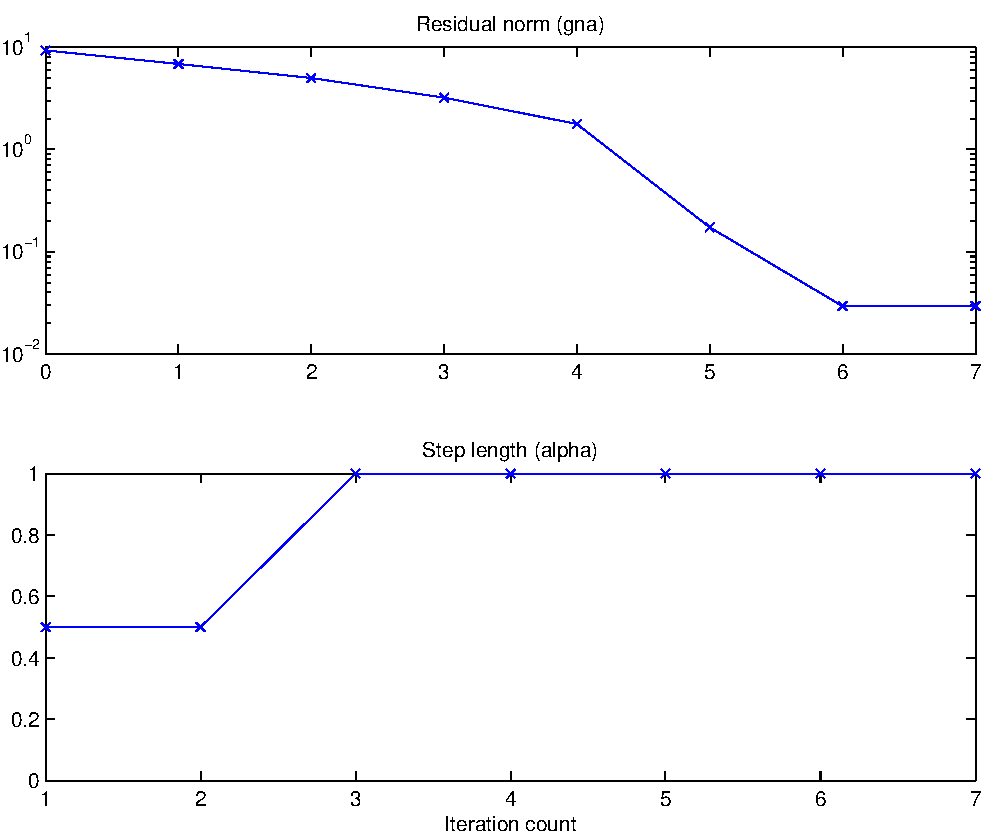
\includegraphics[width=0.5\textwidth]{ill/ccamgnatrace}
  \caption{Residual evolution and damping behaviour during the
    iterations.}
  \label{fig:gnatrace}
\end{figure*}

The final evolution plot, shown in Figure~\ref{fig:gnatrace},
illustrates the evolution of the norm of the total residual and the
damping behaviour, if any, during the bundle iterations. In this
example, the Gauss-Newton-Armijo linesearch damping is active during
the first two iterations. For further details on the damping,
see~\citet{Borlin2013:Bundle}.

\paragraph{Quality plots}

\begin{figure*}
  \centering
  \begin{subfigure}[b]{0.3\textwidth}
    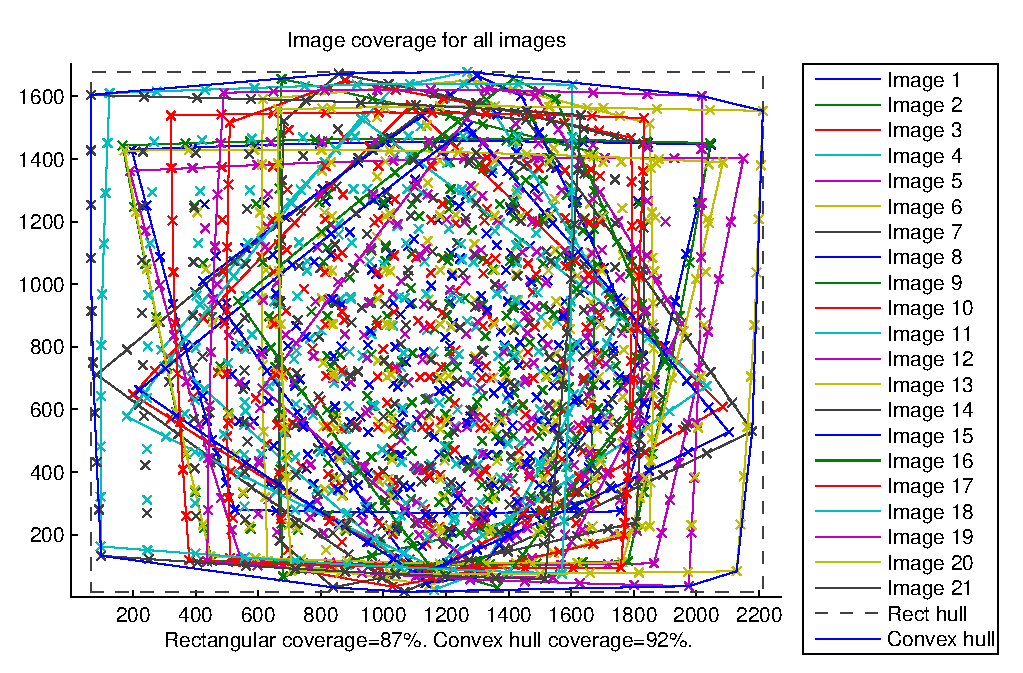
\includegraphics[width=\textwidth]{ill/ccamcoverage}
    \caption{Image coverage}
    \label{fig:ccamCoverage}
  \end{subfigure}%
  \begin{subfigure}[b]{0.3\textwidth}
    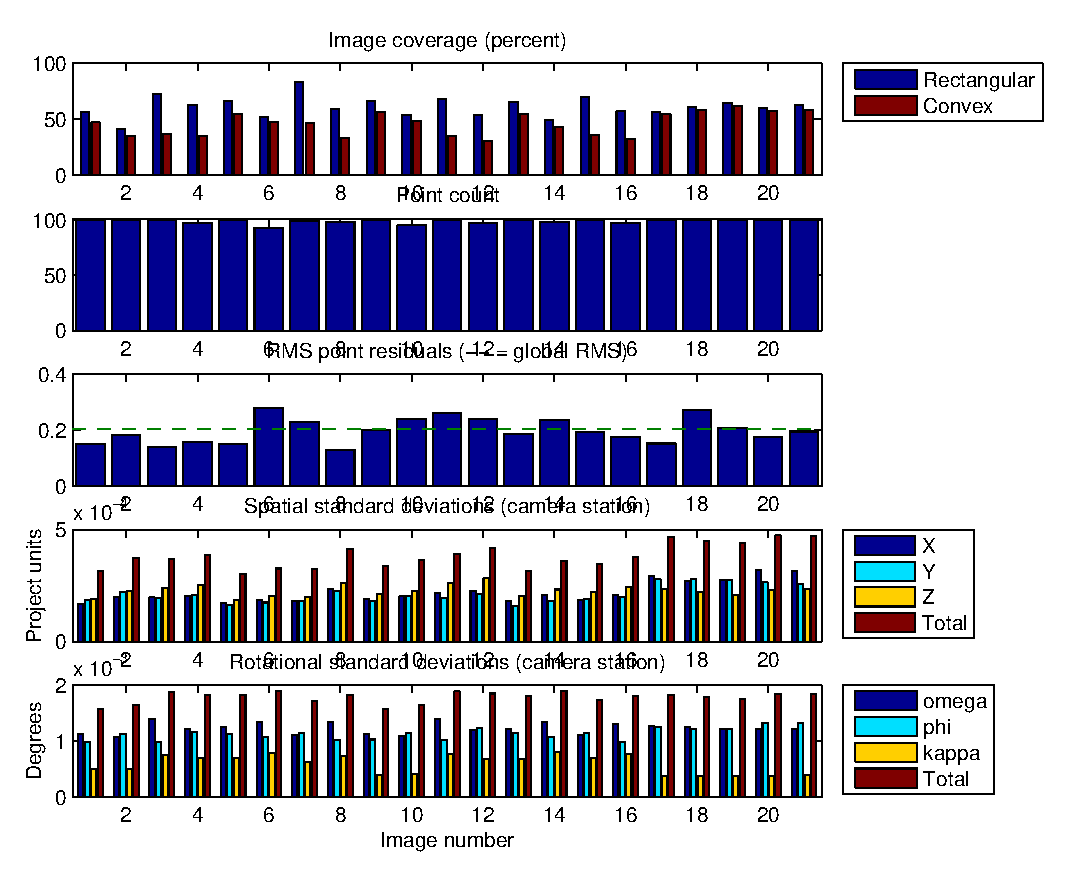
\includegraphics[width=\textwidth]{ill/ccamimstats}
    \caption{Image statistics}
    \label{fig:ccamImstats}
  \end{subfigure}
  \begin{subfigure}[b]{0.3\textwidth}
    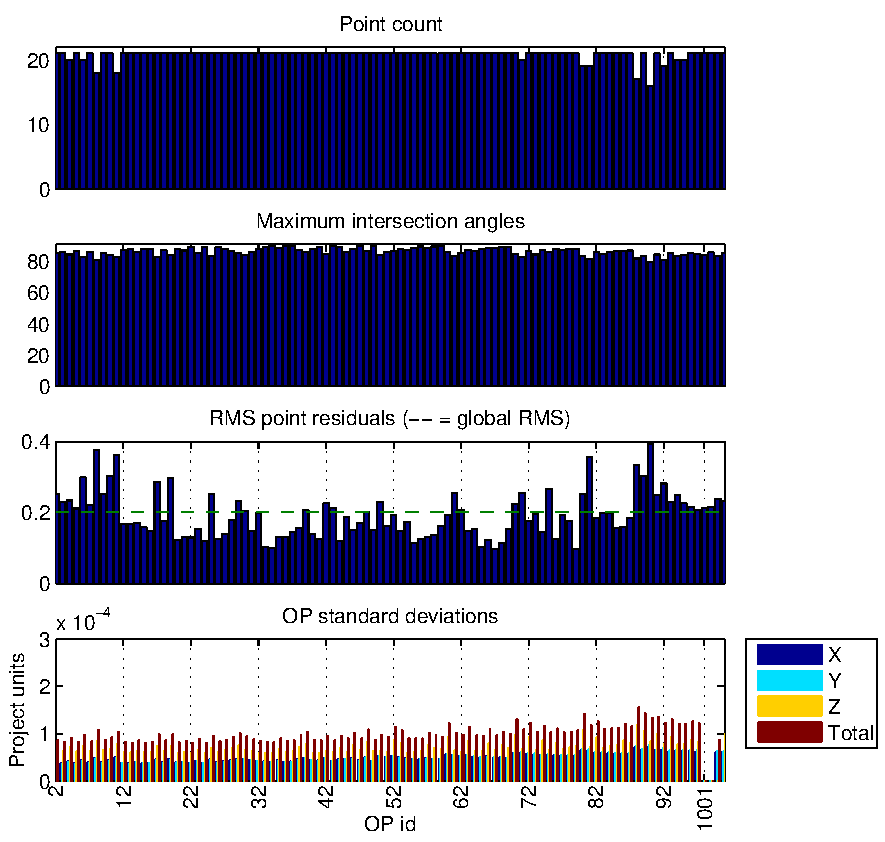
\includegraphics[width=\textwidth]{ill/ccamopstats}
    \caption{Object point statistics}
    \label{fig:ccamOPstats}
  \end{subfigure}
  \caption{Plots of input/output statistics.}\label{fig:ccamQuality}
\end{figure*}

The quality plots a gathered in Figure~\ref{fig:ccamQuality}.
Per-image quality statistics is shown in Figure~\ref{fig:ccamImstats}.
The statistics presented for each image are the image coverage; the
number of measured points; the average (RMS) point residual; and the
standard deviations for the EO parameters for the camera stations. In
this example, the data does not give any obvious support to exclude
the suspected image~21 from the calibration.

The image coverage is detailed in a separate
Figure~\ref{fig:ccamCoverage}. The plotted data is selectable. All
observations from a specific image, including their convex hull, will
be highlighted when a point or line is selected.

Finally, the per-OP quality statistics in Figure~\ref{fig:ccamOPstats}
show the number of observations per OP; the maximum ray intersection
angle; the average (RMS) point residual; and the OP coordinate
standard deviation. The presentation may be zoomed to show only a
subset of the OPs by activating the ``zoom'' function of the figure
window.

\paragraph{Result file}

The result file is modelled after the Photomodeler result file.
The result file is listed in Appendix~\ref{sec:resultFile}.

\subsubsection{romabundledemo}

The \texttt{romabundledemo} function loads the project from
Section~\ref{sec:loadroma} and present essentially the same plots and
the \texttt{camcaldemo}. This demo uses the Photomodeler file as input
to the bundle adjustment that runs a few iterations until convergence.
The same result file and result plots as \texttt{camcaldemo} are
essentially generated. Since the project is larger (60 cams/26~000
points) than the previous example (20 cams/100 points), the
computation will take a bit longer. Computation time was around one
minute running on a HP compaq dc7800 with an Intel Core2 Quad CPU
Q9300 @ 2.50GHz under 64-bit Ubuntu 12.04 (kernel 3.5.0-45).

\subsection{Using your own data}

This section describes how to import you own data using Photomodeler
text export files. If you have another type of input file, you may be
able to write your own loader. Otherwise, if you have a text file you
wish to import, feel free to mail the file to the the toolbox authors
and request an import function. Althought we cannot guarantee
anything, we may adhere to the request, time permitting.

\subsubsection{Export from Photomodeler}

To import a Photomodeler project into the toolbox, the following
steps are valid in Photomodeler Scanner 2012:

\begin{enumerate}
\item Export the project using the \emph{Export Text File} menu
  command. If the command is not available, follow the instructions in
  Appendix~\ref{sec:enableTextExport}.
\item After export, open the \emph{Project/Cameras...} dialog and
  select the camera that was used in your project.
\item Open the generated text file in a text editor.
  \begin{enumerate}
  \item On the 2nd line (usually reading \texttt{0.00005 20}), append
    the width and height in pixels of your images, e.g. to
    \texttt{0.000500 20 5616 3744}.
  \item Inspect the 4th line. For instance,
    the original data in \texttt{roma.txt} was (some trailing zeros removed):

    \texttt{24.3581 18.1143 12.0 35.96404 24.0 0.00022 -0.0 0.0 0.0 0.0}

    The values correspond to the following camera parameters:

    \texttt{focal pp\_x pp\_y format\_w format\_h K1 K2 K3 P1 P2}.

    Notice that most of the significant digits of K1--K3 were lost in
    the text export.
  \item Update the parameter values on the 4th line with values from
    the camera dialog \emph{for each parameter with a larger number of
      significant digits in the dialog}. This usually means all
    parameters except \texttt{format\_w}. In the \texttt{roma.txt}
    test case, the 4th line was modified to:

    \texttt{24.3581 18.1143 12 35.96404 24 2.174e-4 -1.518e-7 0 0 0}.

  \end{enumerate}
\end{enumerate}

\subsubsection{Loading into Matlab}

\begin{enumerate}
\item In matlab, run step~\ref{step:dbatInit} from
  Section~\ref{sec:install} if not already done.
\item \sloppy Set the variable \texttt{fName} to the text export file name \texttt{fName='c:/path/to/exported/file.txt';}, or
  select it using \texttt{[f,p]=uigetfile('*.txt'); fName=[f,p];}
\item Run the \texttt{loadplotdemo} script. A figure with your camera
  network, aligned with the first camera and rotated to have +Z 'up',
  should now have been generated.
\end{enumerate}

\newpage
\bibliography{ref}

\appendix

\newpage

\section{Enabling text export from Photomodeler}
\label{sec:enableTextExport}.

Some versions of Photomodeler do not have the text file export option
enabled by default. In that case, the following steps worked in
Photomodeler Scanner 2012:
\begin{enumerate}
\item Right-click on the main window toolbar, select \emph{Customize toolbar...}.
\item In the \emph{Commands} tab, select the \emph{File} category.
\item Drag the \emph{Export Text File...} command to a toolbar of
  your choice.
\item Now you should be able to export your project as a text file by
  clicking on the \emph{Export Text File} button.
\end{enumerate}


\section{Camera model}

Currently, the only supported camera model is the omega-phi-kappa
Euler angle camera model \citep[Ch.~2.1.2.3]{McGlone2004:Manual} with
the \citet{Brown1971:Close-range} lens distortion model.

\section{Result file example}
\label{sec:resultFile}

\scriptsize
\verbatiminput{ill/C4040Z-2272x1704_result_file.txt}

\end{document}
